%%%%%%%%%%%%%%%%%%%%%%%%%%%%%%%%%%%%%%%%%
% University Assignment Title Page 
% LaTeX Template
% Version 1.0 (27/12/12)
%
% This template has been downloaded from:
% http://www.LaTeXTemplates.com
%
% Original author:
% WikiBooks (http://en.wikibooks.org/wiki/LaTeX/Title_Creation)
%
% License:
% CC BY-NC-SA 3.0 (http://creativecommons.org/licenses/by-nc-sa/3.0/)
% 
% Instructions for using this template:
% This title page is capable of being compiled as is. This is not useful for 
% including it in another document. To do this, you have two options: 
%
% 1) Copy/paste everything between \begin{document} and \end{document} 
% starting at \begin{titlepage} and paste this into another LaTeX file where you 
% want your title page.
% OR
% 2) Remove everything outside the \begin{titlepage} and \end{titlepage} and 
% move this file to the same directory as the LaTeX file you wish to add it to. 
% Then add \input{./title_page_1.tex} to your LaTeX file where you want your
% title page.
%
%%%%%%%%%%%%%%%%%%%%%%%%%%%%%%%%%%%%%%%%%
\title{ \huge \bfseries Q-ant \& Q-gen}
%----------------------------------------------------------------------------------------
%	PACKAGES AND OTHER DOCUMENT CONFIGURATIONS
%----------------------------------------------------------------------------------------

\documentclass[10pt]{article}
\usepackage[english]{babel}
\usepackage[utf8x]{inputenc}
\usepackage{amsmath}
\usepackage{graphicx}
\usepackage[colorinlistoftodos]{todonotes}
\usepackage{hyperref}
\usepackage{booktabs,array}
\usepackage{tabto}
\usepackage{systeme, mathtools}
\usepackage[margin=3cm]{geometry}
\usepackage{enumitem}

\renewcommand{\floatpagefraction}{.9}
%\usepackage[autostyle]{csquotes}
%\MakeOuterQuote{"}
\begin{document}

\begin{titlepage}

\newcommand{\HRule}{\rule{\linewidth}{0.5mm}} % Defines a new command for the horizontal lines, change thickness here

\center % Center everything on the page
 
%----------------------------------------------------------------------------------------
%	HEADING SECTIONS
%----------------------------------------------------------------------------------------

\textsc{\LARGE Università degli studi di Milano-Bicocca}\\[1cm] % Name of your university/college
\textsc{\Large Decision Models}\\[0.3cm] % Major heading such as course name
\textsc{\large Final Project}\\[0.1cm] % Minor heading such as course title

%----------------------------------------------------------------------------------------
%	TITLE SECTION
%----------------------------------------------------------------------------------------
\HRule \\[0.4cm]
%\maketitle
{ \huge \bfseries An Hybrid Metaheuristic Approach to the Traveling Salesman Problem }\\[0.4cm] % Title of your document
\HRule \\[1.5cm]
 
%----------------------------------------------------------------------------------------
%	AUTHOR SECTION
%----------------------------------------------------------------------------------------

\large
\emph{Authors:}\\
Dario Bertazioli-847761-d.bertazioli@campus.unimib.it \\   % Your name
Fabrizio D'Intinosante-838866-f.dintinosante@campus.unimib.it \\
Massimiliano Perletti-847548-m.perletti2@campus.unimib.it\\[1cm] % Your name
% If you don't want a supervisor, uncomment the two lines below and remove the section above
%\Large \emph{Author:}\\
%John \textsc{Smith}\\[3cm] % Your name

%----------------------------------------------------------------------------------------
%	DATE SECTION
%----------------------------------------------------------------------------------------

{\large \today}\\[2cm] % Date, change the \today to a set date if you want to be precise

%----------------------------------------------------------------------------------------
%	LOGO SECTION
%----------------------------------------------------------------------------------------


\includegraphics[scale=0.15]{figs/logo_uni.png}\\[1cm] % Include a department/university logo - this will require the graphicx package

%----------------------------------------------------------------------------------------

\vfill % Fill the rest of the page with whitespace

\end{titlepage}
\begin{abstract}
The ABSTRACT is not a part of the body of the report itself. Rather, the abstract is a brief summary of the report contents that is often separately circulated so potential readers can decide whether to read the report. The abstract should very concisely summarize the whole report: why it was written, what was discovered or developed, and what is claimed to be the significance of the effort. The abstract does not include figures or tables, and only the most significant numerical values or results should be given.
The ABSTRACT is not a part of the body of the report itself. Rather, the abstract is a brief summary of the report contents that is often separately circulated so potential readers can decide whether to read the report. The abstract should very concisely summarize the whole report: why it was written, what was discovered or developed, and what is claimed to be the significance of the effort. The abstract does not include figures or tables, and only the most significant numerical values or results should be given.
\end{abstract}
\vspace*{2cm}
\tableofcontents

\newpage
\section{Introduction}
%The introduction should provide a clear statement of the problem posed by the project, and why the problem is of interest. It should reflect the scenario, if available. If needed, the introduction also needs to present background information so that the reader can understand the significance of the problem. A brief summary of the hypotheses and the approach your group used to solve the problem should be given, possibly also including a concise introduction to theory or concepts used later to analyze and to discuss the results.
\paragraph{The problem:}
the travelling salesman problem (TSP) is an algorithmic problem tasked with finding the shortest route between a set of points and locations that must be visited. 
In the problem statement, the points are the cities a salesperson might visit. The salesman‘s goal is to keep the distance travelled as low as possible. 
TSP has been studied for decades and several solutions have been theorized. 
The simplest solution is to try all possibilities, but this is also the most time consuming and expensive method. 
Many solutions use heuristics, which provides probability outcomes. 
It must be considered that the results are approximate and not always optimal. 
\paragraph{Our approach:}
in this project we tried to apply two meta-heuristics named \textit{Ant Colony Optimization} and \textit{Genetic Algorithm}, implementing their "classical" version and a custom one integrating \textit{Reinforcement Learning Algorithm}, namely \textit{Q-learning} and \textit{Clustering algorithm}, in particular \textit{K-Means} respectively for the first and the second one.

\section{Theoretical context}
In this work we focus on two different approaches to the TSP: implementing some algorithms of the ``Ant-type", and some Evolutionary Algorithms.

\subsection{Ant Family Algorithms}
The former approach is based on the exploitation of a set of algorithms called ``Ant-Family".
\subsubsection{Ant Colony Optimization}
The first type of ``Ant-like" algorithm we implement is the \textbf{Ant Colony Optimization} (ACO) algorithm.

The procedure draws inspiration from a ``real"  Ant  Colony. 
In nature, such a system is  known  to  accomplish  some  difficult  tasks,  being beyond  the capabilities  of  a  single  ant,  exploiting the individuals collaborating  with  each  other.  

In particular, ACO algorithm  is based on  foraging  behaviour  of  some  ant species.  
This behaviour  can  be  summed up as  their  ability  to  find  the  shortest  paths between  a source of food  and  their  nest.
The cooperation  among  the  ants  has inspired researchers to apply a similar collaboration based algorithm to those problems whose   solutions   can   be formulated as a least cost path between an origin and a destination.
Since most optimisation problems  might have such a formulation,  those kind of algorithms are  pretty interesting.

The first ACO algorithm, Ant System, was proposed by Dorigo \cite{cinque, sei, sette, otto, nove}.

It consists in a multi-agent approximate approach that it is said it can produce good-quality solutions in a reasonable time for combinatorial optimisation problems \cite{cinque}. 
The author demonstrate the performance of this algorithm on Travelling Salesman  Problem  (TSP) \cite{sei}. 

Regarding the basic mechanism of ACO, here follows a quick biological explaination.
Ant species are almost blind, thus they interact with the environment and communicate with each  other  expliting the hormones  they  release.  
In partiuclar some  ant  species use a special kind of hormone called \textbf{pheromone}: they lay pheromone trails on the paths they explore, these traces act as stimuli and other ants belonging to the colony are attracted to follow  the  paths  that  have  relatively  more  tracked.  
Due to this mechanism, an individual who is following a  path  because of the  pheromone  trail  also reinforces  it  by  dropping its  own pheromone  too.  

Thus, the  more ants  follow  a  specific  path,  the  more  likely  that  path  becomes  to  be  followed  by  the  ants  in the colony \cite{ cinque,otto, nove}.  

ACO  algorithm  makes use  of ant-like  agents  called artificial ants, that construct their   solutions   collaboratively   by   sharing   their experience on the quality of solutions that were generated so far.
The pheromone trails play  a  leading  role  in  the  utilization  of collective experience.
The solutions are built iteratively.
Artificial  ants  have  ``memory"  to  store  the  path  they  followed  while  constructing  their solutions.  Exploiting such a memory,  typically (even though depending on the speficic class of ant colony algorithm) artificial  ants  do not deposit  the pheromone until they have constructed their solution. Then, They determine the amount of pheromone according  to  the  quality  of  their  solution  and upload the pheromone matrix (the data structure in which the pheromone amount for each part of the total path is stored). 
Automatically, the  paths  belonging  to  better  solutions,  receive  more pheromone.

In iteratively building a solution (a total path) for a single ant, a  local  stochastic  transition  policy  is typically applied, stating how to decide the next node to visit in a graph. Artificial  ants  make  their  decisions  and  transitions  to  their  next  state  in  discrete  time steps, deciding whether to follow the main trails, or to random explore a new path (in our implementation, such a decision is made by a random number generation and imposing a threshold).
Exploration  is  also encouraged  by  a mechanism of  pheromone  evaporation, which prevents the  colony from  getting  stuck  into a solution  corresponding to a (only) local optimum (note however that in  real  ant  colonies  pheromone evaporation is too slow to be a significant part of their search mechanism).

Summing up, Ant Colony Optimisation is a metaheuristic proposed to solve hard optimisation problems. 
The ACO metaheuristic, from a high-level view, is composed of 3 main    stages:    
\begin{itemize}
\item ConstructAntSolutions:
the  artificial  ants  construct  their  solutions.  The transition policy controls  the  ants’  next step to one of the adjacent nodes. Once the ants have completed  their  path,  the quality  of  the current solution is evaluated,  and used in the next step. 
The decision policy is based on following a probability distribution of the type \cite{cinque}:

\begin{equation}
p_{ij}^k=  \frac{[\tau_{ij}]^{\alpha}[\eta_{ij}]^{\beta}}{\sum_{l \in N_i^k} ~  [\tau_{il}]^{\alpha}[\eta_{il}]^{\beta}} ~~~\rm{if} ~j \in N_i^k
\label{eq:prob-aco}
\end{equation}

where 
\begin{itemize}

\item $\eta_{ij}$ indicates an heuristic value specified according to the problem (in the TSP case, is equal to $1/d_{ij}$,
\item  $\tau_{ij}$ is the pheromone quantity on the path between the $i$-th and $j$-th nodes,
\item $\alpha$ and $\beta$ are the parameters used to set the relative importance of the pheromone trail and the heuristic  value.
As $\alpha \rightarrow 0$,  the pheromone  track become  less  important  and  the  ants tend  to choose the closest cities, resulting in a much more ``greedy" search. 
Viceversa, when $\beta \rightarrow 0$, heuristic values are almost ignored and only the tracks are considered in the decision making.  
\end{itemize}
\item UpdatePheromones:  the   pheromone   trails   are   adjusted   based   on   the   latest iteration of  the  colony search process.  
Two different updates happen: 
\begin{itemize}
\item the pheromone  evaporates according to the equation:
\begin{equation}
\tau_{ij}= (1-\rho) \tau_{ij}
\end{equation} 
where $\rho$ is the evaporation coefficient.

\item new pheromone is deposited on the followed path.  The  amount  of  pheromone  to  deposit  is  typically decided  according  to  the  quality  of  the particular  solutions  that  each  path  belongs  to:

\begin{equation}
\Delta \tau_{ij}= \sum_{k=1}^{m} \Delta \tau_{ij}^k
\label{eq:delta-tau}
\end{equation} 
where $\Delta \tau_{ij}^k$ is the pheromone increase amount deposited by the $k$-th ant, which can be (e.g. in Dorigo initial work) taken either as a constant, or $\Delta \tau_{ij}= 1/L_k$, where $L_k$ is the $k-th$ ant path lenght.

However  the entity of  pheromone  update and  it's weight on how the search will be biased towards the best solution found so far is an implementation decision.
\item the following equations can be combinated in:
\begin{equation}
\tau_{ij}= (1-\rho) \tau_{ij} + \Delta \tau_{ij}
\label{eq:aco-update}
\end{equation}
\end{itemize}
\end{itemize}

The pseudocode of the ACO solution is presented in Tab.~\ref{tab:aco-pseudo}.

\begin{table}
\centering
\scalebox{0.8}{
\begin{tabular}{@{}>{\hspace{3em}}p{.8\linewidth}@{}}
\toprule
\unskip \textbf{Algorithm 1} Ant Colony Optimization \\
[.25\normalbaselineskip]
\textbf{Main Algorithm}\\[.25\normalbaselineskip]
{\footnotesize 0:} initialize best\_dist and best\_path to None\\
{\footnotesize 1:} \textbf{for} generation \textbf{in} generations: \\
{\footnotesize 2:} \quad create n\_ants artificial ants  \\
{\footnotesize 3:} \quad \textbf{for} one\_ant \textbf{in} ants: \\
{\footnotesize 4:} \qquad make a single ant path (see Make path)\\
{\footnotesize 5:} \qquad compute the path length \\
{\footnotesize 6:} \qquad update best\_dist and best\_path \\
{\footnotesize 7:} \quad update the pheromon matrix\\
\quad ~~ (local update only for child processes, according to eq.~\ref{eq:aco-update}) \\
{\footnotesize 8:} \quad every a certain n of iterations:\\
{\footnotesize 9:} \qquad update the global pheromone matrix\\
\qquad ~~~(shared in MPI environment among master\&child.)\\
{\footnotesize 10:} \textbf{return} best\_dist, best\_sol \vspace*{0.2cm}\\
[.25\normalbaselineskip]
\textbf{Make path}\\[.25\normalbaselineskip]
{\footnotesize 1:} start from a vertex \\
{\footnotesize 2:} add start vertex to visited nodes \\
[.25\normalbaselineskip]
{\footnotesize 3:} \textbf{for} each remaining vertex: \\
{\footnotesize 4:} \quad list the neighbors \\
{\footnotesize 5:} \quad list the not yet visited neighb \\
{\footnotesize 6:} \quad calculate the probability of choosing a vertex (according to eq.~\ref{eq:prob-aco})\\
{\footnotesize 7:} \quad choose the vertex according to probability \\
{\footnotesize 8:} \quad add the choosen vertex to the visited list \\
{\footnotesize 9:} \quad return the chosen vertex id \vspace*{0.2cm}\\
[.25\normalbaselineskip]
\textbf{Local update pheromon matrix}\\[.25\normalbaselineskip]
{\footnotesize 1:} \textbf{for} ant \textbf{in} ant\_colony : \\
{\footnotesize 2:} \quad \textbf{for} each vertex of one\_ant\_path : \\
{\footnotesize 3:} \qquad increase pheromon\_matrix between current and next vertex of $\Delta \tau$\\
\qquad ~~~(according to eq.~\ref{eq:aco-update}) \vspace*{0.2cm}\\
[.25\normalbaselineskip]
\textbf{Global update pheromon matrix (parallelism)}\\[.25\normalbaselineskip]
{\footnotesize 1:} gather from MPI env all the pheromone matrices\\
{\footnotesize 2:} \textbf{if} process is the parent process (rank==0): \\
{\footnotesize 3:}\quad for each element average over the n\_cores matrices. \\
{\footnotesize 4:} broadcast obtained pheromone matrix to the other \\
\quad processes \\
\bottomrule
\end{tabular}
}
\caption{\label{tab:aco-pseudo}Ant Colony pseudocode}
\end{table}
 
\subsubsection{Ant-Q Metaheuristic}
In order to better understanding the working mechanism of Ant-Q Metaheuristic and to give deeper insight in our implentation (following \cite{undici} ), let us introduce some theoretical hints for the context.
\paragraph{Hints on reinforcement learning:}
Reinforcement  Learning  (RL)  is  an  (almost) unsupervised  learning  approach.

It consists of an  \textbf{agent}  who tries to learn how  to  reach  a  goal  by  a continuous interaction with  the environment. 
There is an evaluation phase where the quality of agent's actions is considered and feedbacks to the agent are given in the form a numerical reward. 
This type of feedback is known as evaluative feedback: in contrary of supervised learning, here the agent is not explicitly told what action is the best to take  in  a  certain  situation, whereas it should  try  a set of possible actions and learn the best strategy yielding the most reward itself.  

In some cases, the goal state (that is, the agent reaching its objective) can be obtained only after a sequence of actions: as a result the reward is delayed (FIXME: cfr section ant q delayer reward). 

Summing up, and according to \cite{diciotto}, the  RL  problem  can  be  defined  as  the  problem  of  an agent  interacting  with  a  complex environment trying to maximise its long-run reward over a sequence of discrete time steps.

The agent follows a \textbf{policy} to decide on its action according to the current state and conditions. 

This policy is typically a  stochastic  function ($\pi(s,a)$) that  indicates a probability  of  choosing an action $a$ given a state $s$.
Notice that agent has the possibility to change its initial policy  according  to  new experiences  in order to  achieve  optimal cumulative  reward  over  time.  

The  value  of  a  state $V_\pi(s)$  is  defined  as  the  expected  cumulative reward that  will  be  obtained starting from a state $s$ and acting according to the current policy $\pi$. 
In the same way, the value of  a pair state-action($Q_\pi(s,a)$) is  the  expected  return  obtained starting  from  $s$  with  action $a$  and  then following  the policy. 
In formulas, $V$ is defined as:
\begin{equation}
V^\pi(s)=E_\pi \{ \sum_i \gamma^i r_{t+1, i+1 ~ | s_t=s } \}
\end{equation}

and accordingly:
\begin{equation}
Q^\pi(s,a)=E_\pi \{ \sum_i \gamma^i r_{t+1, i+1 ~|~ s_t=s,~ a_t=a } \}
\end{equation}

The RL problem consists in the agent trying to find the optimal policy $\pi^*$ that maximizes the value  functions, obtaining thus:
\begin{equation}
V^*(s)= max_{a \in A(s)}(Q^{\pi^*}(s,a)
\end{equation} 
however, the policy estimation can be in general a complex problem, and an optimal policy can be obtained with various algorithms, such as Policy Iteration and Value Iteration. There are also kind of learning mechanism defined as ``off-policy", because they do not exploit a proper policy procedure.

\paragraph{Q-Learning}: 
is  an  off-policy  method, meaning  that  it updates the values  iteratively basing this process on  the  action that  gives  the  maximum  value  (that is, such an algorithm tries to directly  learn $Q^*$  instead  of  learning $Q_\pi$ first). In figure~\ref{fig:q_pseudo} it is shown the pseudocode of the algorithm:  the  agent  uses  a  so called $\epsilon$-greedy  policy,  but  updating the  current  value  estimate  considering the  action  that  provides  the  maximum  value  at  the successor state instead of considering the (current-)policy-suggested action. 
\begin{figure}
\centering 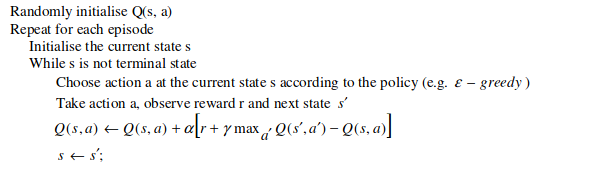
\includegraphics[scale=0.6]{figs/q_pseudo.png}
\caption{\label{fig:q_pseudo} The pseudo code of a typical Q-learning algorithm implementation.}
\end{figure}

\paragraph{Ant-Q Algorithm}:
one of the core points of this project consists in the implementation of the Ant-Q algorithm, introduced by Gambarella \cite{undici} in collaboration with Dorigo, attempting to ameliorate the ``classic" ACO performances.  

In this approach, the pheromone update rule  is borrowed from the Q-learning prassi:
\begin{equation}
Q(s,a) \leftarrow (1-\alpha) Q(s,a) + \alpha (r + \gamma [max_{a^{'}} Q(s^{'},a^{'})-Q(s,a)]~.
\label{eq:q-eq}
\end{equation}
In particular, equation \ref{eq:aco-update} is changed into the following: 
\begin{equation}
\tau_{ij}= (1-\alpha) \tau_{ij} + \alpha( \Delta \tau_{ij} + \gamma max_{l\in N^k_j}\tau_{jl}) ~.
\label{eq:antq-eq}
\end{equation} 
(FIXME: fix eq punctuation everywhere)
The next action (what next node connecting to) is chosen according to:
\begin{equation}
s = \begin{cases} arg~max_{a \in J_k(s)} [Q(s,a)]^\alpha [\eta(s,a)]^\beta & \mbox{if } q \leq q_0 \\ S & \mbox{otherwise } \end{cases} 
\label{eq:antq-choice}
\end{equation}
where correspondingly to equation \ref{eq:prob-aco}, $\eta$ is an heuristic value associated with the inverse of distance between a pair of nodes, and $\alpha~, \beta$ are weight-parameters for the interaction.

Comparing equation~\ref{eq:antq-eq} to to the Q-learning update rule \ref{eq:q-eq} , it is worth to notice that :
\begin{itemize}
\item  equation~\ref{eq:antq-eq}  updates the pheromone  value  of  the  transition  ($i$, $j$)  according to the  pheromone  value  of  the  next transition  ($j$, $ l$),
\item equation~\ref{eq:antq-eq} uses  the second part of equation \ref{eq:q-eq} (known as TD Error) to  weight the  pheromone  quantity associated  to  the current  edge  with  a learning  rate $\alpha$  and  a discount  rate $\gamma$, 
\item the equation 
\begin{equation}
\tau_{ij}= (1-\alpha) \tau_{ij} + \alpha(\gamma max_{l\in N^k_j}\tau_{jl}) 
\label{eq:localupd}
\end{equation}
is used for the pheromon matrix update (namely a local update) during each path construction (of each ant), and it does not include the delayed reward $\Delta \tau_{ij}$,
\item $\Delta \tau_{ij}$ is calculated according to the solution quality, as anticipated circa equation \ref{eq:delta-tau}, and assigned in a ``delayed" mode: thus the value of $\Delta \tau_{ij}$  for all $i$ and $j$ will be $0$ while the ants  apply  the  update  rule \ref{eq:localupd}  during  their  construction  of the  current solution. 
Therefore, the update rule \ref{eq:antq-eq}	 is reapplied at the completion of the current solution, but with the value of the next transition considered to be equal to zero. (thus uploading only with $\Delta \tau_{ij}$:
\begin{equation}
\tau_{ij}= (1-\alpha) \tau_{ij} + \alpha(\Delta\tau_{ij}) 
\label{eq:antq-delay}
\end{equation}

\item still according to \cite{undici} \cite{diciotto} $\Delta \tau_{ij}$ can be updated with an iteration  best  rule (update every single colony iteration) or  global  best (update based on the global best value.
\end{itemize}

Notice that many other attempts were made in the direction of hybridizing ACO and reinforcement learning based algorithms, some particularly interesting and successful, such as \cite{quattordici},\cite{quindici},\cite{sedici}. However, due to the few time available, we could head our force in implementing only the in-detail-described Ant-Q.

The pseudocode regarding our implementation of such an hybrid metaheuristic is reported in Tab.~\ref{tab:antq-pseudo}

\begin{table}
\centering
\scalebox{0.75}{
\begin{tabular}{@{}>{\hspace{3em}}p{.8\linewidth}@{}}
\toprule
\unskip \textbf{Algorithm 2} Ant-Q algorithm\\
[.25\normalbaselineskip]
\textbf{Main Algorithm}\\[.25\normalbaselineskip]
{\footnotesize 0:} initialize best\_dist and best\_path to None\\
{\footnotesize 1:} \textbf{for} generation \textbf{in} generations: \\
{\footnotesize 2:} \quad create n\_ants artificial ants  \\
{\footnotesize 3:} \quad \textbf{for} one\_ant \textbf{in} ants: \\
{\footnotesize 4:} \qquad make a single ant path (see Make path)\\
{\footnotesize 5:} \qquad compute the path length \\
{\footnotesize 6:} \qquad update best\_dist and best\_path \\
{\footnotesize 7:} \qquad update ph. matrix with delayed rewards\\
\qquad ~~~(according to eq.~\ref{eq:antq-delay})\\
{\footnotesize 8:} \quad update the global pheromone matrix \\
\quad ~~(shared in MPI environment among master\&child.)\\
{\footnotesize 9:} \textbf{return} best\_dist, best\_sol \\
[.25\normalbaselineskip]
\textbf{Make path}\\[.25\normalbaselineskip]
{\footnotesize 1:} start from a vertex \\
{\footnotesize 2:} add start vertex to visited nodes \\
[.25\normalbaselineskip]
{\footnotesize 3:} \textbf{for} each remaining vertex: \\
{\footnotesize 4:} \quad list the neighbors \\
{\footnotesize 5:} \quad list the not yet visited neighb \\
{\footnotesize 6:} \quad generate a random number $q \in \{0,1\}$\\
{\footnotesize 7:} \quad if q < q\_0: (threshold)\\
{\footnotesize 8:} \qquad select next vertex according to eq.~\ref{eq:antq-choice}\\
{\footnotesize 9:} \quad else: \\
{\footnotesize 10:}\qquad calculate the probability of choosing a vertex \\
{\footnotesize 11:}\qquad (according to eq.~\ref{eq:prob-aco})\\
{\footnotesize 12:} \qquad choose the vertex according to probability \\
{\footnotesize 13:} \quad add the choosen vertex to the visited list \\
{\footnotesize 14:} \quad give local rewards (local update pheromone matrix) \\
{\footnotesize 15:} \quad return the chosen vertex id \\
[.25\normalbaselineskip]
\textbf{Local update pheromone matrix}\\[.25\normalbaselineskip]
{\footnotesize 1:} \textbf{for} ant \textbf{in} ant\_colony : \\
{\footnotesize 2:} \quad \textbf{for} each vertex of one\_ant\_path : \\
{\footnotesize 3:} \qquad increase pheromon\_matrix between current \\
\qquad ~~and next vertex of a $\Delta \tau$ (according to eq.~\ref{eq:antq-eq})\\
[.25\normalbaselineskip]
\textbf{Global update pheromon matrix (parallelism)}\\[.25\normalbaselineskip]
{\footnotesize 1:} gather from MPI env all the pheromone matrices\\
{\footnotesize 2:} \textbf{if} process is the parent process (rank==0): \\
{\footnotesize 3:}\quad for each element average over the n\_cores matrices. \\
{\footnotesize 4:} broadcast obtained pheromone matrix to the other \\
\quad processes \\
\bottomrule
\end{tabular}
}
\caption{\label{tab:antq-pseudo}Ant-Q pseudocode}
\end{table}

\paragraph{Parallel Implementation:} since both the ACO and Ant-Q are memory and computational-expensive, we suggest a parallel implementation of each algorithm.

The type of proposed algorithm is naturally easy to code in a parallel implementation, being enough to split the total number of ants into a number of sets (called \textit{n\_ants\_per\_core} in the code) of ants that will be distributed on each single core.

Thus, a parent process initializes the algorithm, creating n\_core childs each operating on a "personal" memory area. 
Thus, every child has its own data structures, in particular its own pheromone matrix. 
The MPI/OpenMPI\footnote{\url{https://www.open-mpi.org/}} \footnote{a nice introduction to MPI basic usage: \url{https://princetonuniversity.github.io/PUbootcamp/sessions/parallel-programming/Intro_PP_bootcamp_2018.pdf}} software (in partiicular mpi4py\footnote{https://mpi4py.readthedocs.io/en/stable/}, a pythonic Api for OpenMPI) is used to host a shared pheromone matrix which will be updated according to the pseudocode in tab.~\ref{tab:aco-pseudo},\ref{tab:antq-pseudo} (as a mean-matrix), and which every ``local" matrix will be update to after every iteration, so that every artificial ant in every child process will ``feel" a as similar as possible pheromone effect.

\subsection{Evolutionary Algorithms}
\subsubsection{Genetic Algorithm}
The latter approach we faced along this work is the \textbf{Genetic Algorithm}, which we initially implement in its classical version.
This algorithm is based on a biological metaphor: the resolution of a problem is seen as a competition among a population whose evolving individuals become better and better candidates solutions over time. 
A “fitness” function is used to evaluate each individual to decide whether it will contribute to the next
generation. 
Then, in analogy with the biological metaphor (the gene transfer in sexual reproduction), a crossover operator is applied in order to generate the next generation of the population.
This process, according to the evolutionary theory (Darwinism), should lead after a certain number of iterations to a much more fit ensemble of individuals representing ``good" candidate solutions to the considered problem.

%At the beginning of a run of a genetic algorithm, a large population of random chromosomes is created. Each one, when decoded, will represent a different solution to the problem at hand. Some of the advantages of a GA (R. Haupt & S. E. Haupt 2004) include the following: • It optimizes with continuous or discrete variables;• Does not require derivative information;• Simultaneously searches through wide sampling of the cost surface;• Deals with a large number of variables and is well suited for parallel computers;• Optimizes variables with extremely complex cost surfaces (they can jump out of alocal minimum);• Provides a list of optimum variables, not just a single solution;• May encode the variables so that the optimization is done with the encodedvariables; and• Works with numerically generated data, experimental data, or analyticalfunctions.A typical genetic algorithm presents the following operators:• Crossover - this operator is used to vary the population of the chromosomes fromone generation to the next. It selects the two fittest chromosomes in the populationand produces a number of offspring. There are several crossover techniques; in thiswork, we will use the one-point crossover.• Selection - this operator replicates the most successful solutions found in apopulation at a rate proportional to their relative quality, which is determined bythe fitness function. In this paper we will use the roulette wheel selection techniquefor this operator.• Mutation - used to maintain genetic diversity from one generation of a populationof chromosomes to the next. It selects a position of an offspring chromosome withsmall probability and changes the value based on the problem model; for example,in this work, the mutation operator modifies the offspring chromosome simply bychanging the position of a gene.
The pseudo code of the standard genetic algorithm is summarized in the Tab.~\ref{Tab: GA pseudocode}, where Tm is the mutation rate that determines the rate at which the mutation operator is applied, Tp is the population size (number of
chromosomes) and MaxG the number of generations used in the experiment\cite{venti}.
\begin{table}
\centering
\begin{tabular}{@{}>{\hspace{3em}}p{.8\linewidth}@{}}
\toprule
\unskip \textbf{Algorithm 3} Genetic Algorithm\\
{\footnotesize 1:} \textbf{procedure} Genetic(Tm,Tp,MaxIt)\\[.25\normalbaselineskip]
{\footnotesize 2:}\quad $Pop \leftarrow GeneratePopulation(Tp)$ \\
{\footnotesize 3:}\quad $Pop \leftarrow Evaluation(Pop)$ \\
{\footnotesize 4:}\quad \textbf{for} $i = 1\dots MaxIt$ \textbf{do} \\
{\footnotesize 5:}\qquad $Pop \leftarrow Selection(Pop)$ \\
{\footnotesize 6:}\qquad $Pop \leftarrow Crossover(Pop)$ \\
{\footnotesize 7:}\qquad $Pop \leftarrow Selection(Pop)$ \\
{\footnotesize 8:}\qquad With probability $Tm$ do: \\
{\footnotesize 11:}\qquad $Pop \leftarrow Mutation(Pop)$ \\
{\footnotesize 12:}\quad \textbf{end for} \\
{\footnotesize 13:} \quad \textbf{return} the best solution in $Pop$ \\
{\footnotesize 14:} \textbf{end procedure} \\
\bottomrule
\end{tabular}
\caption{\label{Tab: GA pseudocode}Genetic Algorithm pseudocode}
\end{table}
Finally, with the aim to explore a new variation of the standard algorithm, we try to integrate a \textit{Clustering algorithm} named \textit{K-Means} in order to reduce the problem dimension and improve the genetic procedure performance.

\subsubsection{KGA Metaheuristic}
The \textbf{K-Means Genetic Algorithm} (KGA) is composed by different phases described below.

\paragraph{Clustering with K-Means:} At first, specifically for the TSP problem, we need to cluster our cities into close groups with a clustering method.

The \textit{K-Means} method is designed to partition a set of data into \textit{K} classes with \textit{K} chosen as desired.
This method constructs partitions of the data-matrix so that the squared Euclidean distance between the row vector for any object and the centroid vector of its respective cluster is at least as small as the distances to the centroids of the remaining clusters.
The centroid of cluster $C_k$ is a point in $P$-dimensional space found by averaging the values on each variable over the objects within the cluster. For instance, the centroid value for $j$th variable in cluster $C_k$ is
\begin{equation}
\bar{x}_{j}^{(k)} = \frac{1}{n_k} \sum_{i \in C_k} x_{ij}
\end{equation}
and the complete centroid vector for cluster $C_k$ is given by\cite{ventidue}
\begin{equation}
\bar{x}^{(k)}  = (\bar{x}_1^{(k)},\bar{x}_2^{(k)},\dots,\bar{x}_p^{(k)})
\end{equation}
\begin{table}
\centering
\begin{tabular}{@{}>{\hspace{3em}}p{.8\linewidth}@{}}
\toprule
\unskip \textbf{Algorithm 4} K-Means Algorithm\\
{\footnotesize 1:} Set the K cluster centers randomly; \\[.25\normalbaselineskip]
{\footnotesize 2:} \textbf{repeat} \\
{\footnotesize 3:}\quad \textbf{for} \textit{each vertex} \textbf{do} \\
{\footnotesize 4:}\qquad Calculate distance measure to each cluster; \\
{\footnotesize 5:}\qquad Assign it to the closest cluster; \\
{\footnotesize 6:}\quad \textbf{end} \\
{\footnotesize 7:}\quad recompute the cluster centers positions; \\
{\footnotesize 8:} \textbf{until} stop criteria are met; \\
\bottomrule
\end{tabular}
\caption{\label{Tab: K-Means pseudocode}K-Means pseudocode}
\end{table}
Finally, K-Means clustering algorithm is presented in Tab:~\ref{Tab: K-Means pseudocode}.
\paragraph{Intra-group evolution operation:}
The aim of the intra-group evolution operation is to find the shortest path for the given vertices in each cluster.
GA is performed in each cluster aiming to obtain an approximate solution by a couple of genetic operations like selection, crossover, and mutation.
Running the GA algorithm on smaller portion of original data allows to improve performance and reach better solutions.
Eventually all those clusters could be handled parallel.
The result of this step is tours $T_1,T_2,\dots,T_k$ for clusters $C_1,C_2,…,C_k$.
\paragraph{Inter-group connection:}
In the last step, what we obtain is the shortest path between the given vertices in each cluster.
With the aim to reconstruct the whole shortest path we need to connect properly every cluster to the others.
Connect two clusters determine which edges will be deleted from the adjacent shortest path among each cluster, and which edges will be linked for combining two adjacent clusters into one. 
Assuming $i$ and $j$ are two closest vertices between two clusters $G_i$ and $G_j$ for $G_i,i−1$ and $i+1$ are two adjacent vertices of $i$, and the same to $G_j,j−1$ and $j+1$ are two adjacent vertices of $j$. 
Given $G_i$ and $G_j$, in order to combine the two clusters into one, we need to select two vertices $i \in i′$ and $j \in j'$ for deleting and linking edges.
With the aim to apply this strategy we refer to Eq.~\ref{eq: int-group-conn} 
\begin{equation}
\{i^*,j^*\} = \mathrm{arg min}_{i',j'} 
\begin{cases}
d_{ij} + d_{i'j'} - d_{ii'} - d_{jj'}\\d_{ij'} + d_{i'j} - d_{ii'} - d_{jj'}
\end{cases}
\label{eq: int-group-conn}
\end{equation}
where $i' \in \{i-1; i+1\}, j' \in \{j-1;j+1\}$.
Following this strategy, the first two clusters are combined into one, then the new generated cluster combines with the third cluster, and so on, step by step. At last, all those clusters are joined into one tour, and the shortest whole traveling tour is derived.
The whole process of the KGA is listed in Tab.~\ref{Tab: KGA pseudocode} \cite{ventitre},\cite{ventiquattro}.
\begin{table}
\centering
\begin{tabular}{@{}>{\hspace{3em}}p{.8\linewidth}@{}}
\toprule
\unskip \textbf{Algorithm 5} KGA\\
{\footnotesize 1:} \textbf{input} an TSP;\\[.25\normalbaselineskip]
{\footnotesize 2:} K-Means is adopted to cluster the TSP into k \textit{sub-problems}\\
{\footnotesize 3:} \textbf{For} each sub-prob $i=1$ to $k$, do: \\
{\footnotesize 4:}\quad \textbf{repeat}\\
{\footnotesize 5:}\qquad GA procedure \\
{\footnotesize 6:}\quad \textbf{until} \textit{stop criteria are met} \\
{\footnotesize 7:}\quad \textbf{Output} shortest path for sub-problem $i$;\\
{\footnotesize 8:} \textbf{End}\\
{\footnotesize 9:} Seek for the best combining seq $S$ with GA\\
{\footnotesize 10:} Combine all those shortest path into one tour\\
{\footnotesize 11:} \textbf{Output} the shortest whole travelig tour.\\
\bottomrule
\end{tabular}
\caption{\label{Tab: KGA pseudocode}KGA pseudocode}
\end{table}


\section{Datasets}
The datasets used in this work are taken from  \url{https://wwwproxy.iwr.uni-heidelberg.de/groups/comopt/software/TSPLIB95/tsp/}, a large source of TSP datasets largely cited in literature. 
There are datasets of variable dimension and for everyone is also available the optimal solution so that is possible for us to compare our results with the optimal one. 
Every solution is available at \url{https://wwwproxy.iwr.uni-heidelberg.de/groups/comopt/software/TSPLIB95/STSP.html}. Every dataset is composed by a list of ``\textit{cities}" with two coordinates points; the only preprocessing we apply is to compute a matrix containing the distance between every point and the other ones.

In particular we use 5 datasets of different dimension:
\begin{itemize}[noitemsep]
\item dj38
\item berlin52
\item ch130
\item d198
\item pr1002
\end{itemize}
We have choosen these datasets because they are very used and largely cited in literature allowing us to compare our results with others.
\section{The Methodological Approach}
%This is the central and most important section of the report. Its objective must be to show, with linearity and clarity, the steps that have led to the definition of a decision model. The description of the working hypotheses, confirmed or denied, can be found in this section together with the description of the subsequent refining processes of the models. Comparisons between different models (e.g. heuristics vs. optimal models) in terms of quality of solutions, their explainability and execution times are welcome. 
%Do not attempt to describe all the code in the system, and do not include large pieces of code in this section, use pseudo-code where necessary. Complete source code should be provided separately (in Appendixes, as separated material or as a link to an on-line repo). Instead pick out and describe just the pieces of code which, for example:
%\begin{itemize}
%\item are especially critical to the operation of the system;
%\item you feel might be of particular interest to the reader for some reason;
%\item  illustrate a non-standard or innovative way of implementing an algorithm, data
%structure, etc..
%\end{itemize}
%You should also mention any unforeseen problems you encountered when implementing the
%system and how and to what extent you overcame them. Common problems are:
 %difficulties involving existing software.
\subsection{Ant Algorithms}
Regarding the Ant-Family blabla

\subsection{Evolutionary Algorithms}
%Our implementation of the genetic blabla
% maybe better in methodological approach
As said evolutionary algorithms like \textit{Genetic algorithm} uses operators inspired by natural selection such as reproduction, mutation, recombination and selection.
\textit{Genetic algorithm} is very customizable in every component; in this work we have focused our attention on the selection part.
In particular we tried to apply the following selection strategies \cite{ventuno}:
\begin{itemize}
\item roulette-wheel selection;
\item tournament selection.
\end{itemize}
The \textbf{roulette-wheel} selection consists in giving a weight to each chromosomes (the individuals in our population) and this weight corresponds to a portion of a roulette wheel.
In this way chromosomes with higher fitness will have higher weight and a larger portion of the wheel.
\begin{equation}
p_i = \frac{f_i}{\sum_{j = 1}^n f_j}
\end{equation}
Spinning the wheel for different times allows selecting the individuals for the next generation.
Finally, the roulette wheel is nothing more than a weighted sort mechanism.

The \textbf{tournament} selection, instead, consists in randomly selecting a group of individuals from the larger population and taking only the one with the highest fitness. 
The number of individuals competing in each tournament is commonly set to 2 but in this work we implemented a variable tournament dimension for each iteration.

The other elements, however, have been kept standard.
Among these we remember:
\begin{itemize}
\item \textbf{crossover:} we applied the simplest crossover strategy called \textit{single-point};
\item \textbf{mutation:} we applied the simplest mutation version called \textit{point mutation}, with a mutation probability described by a \textbf{mutation rate}.
\end{itemize}


\section{Results and Evaluation}
The Results section is dedicated to presenting the actual results (i.e. measured and calculated quantities), not to discussing their meaning or interpretation. The results should be summarized using appropriate Tables and Figures (graphs or schematics). Every Figure and Table should have a legend that describes concisely what is contained or shown. Figure legends go below the figure, table legends above the table. Throughout the report, but especially in this section, pay attention to reporting numbers with an appropriate number of significant figures. 

\section{Discussion}
The discussion section aims at interpreting the results in light of the project's objectives. The most important goal of this section is to interpret the results so that the reader is informed of the insight or answers that the results provide. This section should also present an evaluation of the particular approach taken by the group. For example: Based on the results, how could the experimental procedure be improved? What additional, future work may be warranted? What recommendations can be drawn?


\section{Conclusions}
Conclusions should summarize the central points made in the Discussion section, reinforcing for the reader the value and implications of the work. If the results were not definitive, specific future work that may be needed can be (briefly) described. The conclusions should never contain ``surprises''. Therefore, any conclusions should be based on observations and data already discussed. It is considered extremely bad form to introduce new data in the conclusions.

%\section*{References}

%The references section should contain complete citations following standard form.  The references should be numbered and listed in the order they were cited in the body of the report. In the text of the report, a particular reference can be cited by using a numerical number in brackets as %\cite{Lee2015} that corresponds to its number in the reference list. \LaTeX provides several styles to format the references

%\bibliographystyle{IEEEtran}
%\bibliography{references.bib}
\newpage
\begin{thebibliography}{9}
\bibitem{uno}
Blum,  C.,  and  Dorigo,  M.  The  Hypercube  framework  for  Ant  Colony  Optimization. In:IEEE Transactions on Systems, Man, and Cybernetics, Vol. 34, No. 2, April 2004. 
 
\bibitem{due}
Buşoniu,  L.,  Schutter,  B.,  and  Babuska  R.  Learning  and  Coordination  in  Dynamic Multiagent  Systems.  Technical  Report  submitted  to  Delft  University  of  Technology,  Delft Center for Systems and Control, Netherlands, October 2005. 

\bibitem{tre}
Cordon,  O.,  Herrera,  F.,  Fernandez  de  Viana,  I.,  and  Moreno,  L.  A  New  ACO  Model Integrating Evolutionary Computation Concepts: The Best-Worst Ant System. In:  Proc. of ANTS’2000.  From  Ant  Colonies  to  Artificial  Ants:  Second  International  Workshop  on  Ant Algorithms, Brussels, Belgium, September 7-9, pp. 22-29, 2000.

\bibitem{quattro}
Cordon,  O.,  Herrea,  F.,  and  Stützle,  T.  A  Review  on  The  Ant  Colony  Optimization Metaheuristic:  Basis,  Models  and  New  Trends.  In: Mathware  and  Soft  Computing.  Vol.  9, pp.141-175, 2002.

\bibitem{cinque}
Dorigo,  M.,  Maniezzo,  V.,  and  Colorni,  A.  Ant  System:  Optimization  by  a  Colony  of Cooperating Agents. In: IEEE Transactions on Systems, Man, and Cybernetics. Vol. 26, No. 1, 1996.

\bibitem{sei}
Dorigo,  M.,  and  Gambardella,  L.  M.  Ant  Colony  System:  A  Cooperative  Learning Approach  to  the  Travelling  Salesman  Problem.  In: IEEE  Transactions  on  Evolutionary Computation, Vol.1 No.1, pp.53-66, April 1997.

\bibitem{sette}
Dorigo, M., Di Caro, G., and Gambardella, L. M. Ant algorithms for discrete optimisation. In: Artificial Life 5(2),pp.137-172, April 1999. 

\bibitem{otto}
Dorigo, M., and Stützle, T. Ant Colony Optimization, MIT Press, Cambridge, MA, 2004.

\bibitem{nove}
Dorigo,  M.,  Birattari,  M.,  and  Stützle,  T.  Ant Colony  Optimization:  Artificial  Ants  as  a Computational   Intelligence   Technique.  In: IEEE  Computational  Intelligence  Magazine, November 2006.

\bibitem{undici}
Gambardella, L. M. and Dorigo, M. Ant-Q: A Reinforcement Learning Approach to the Traveling Salesman Problem. In: Proc. ML-95, 12th Int. Conf. Machine Learning. Palo Alto, CA: Morgan Kaufmann, pp. 252–260, 1995.

\bibitem{diciotto}
Sutton,  R.  S.,  and  Barto,  A.  G. Reinforcement  Learning:  An  Introduction.  MIT  Press, Cambridge, MA, 1998.

\bibitem{sedici}
Sun,  R.,  Tatsimu,  S.,  Zhao,  G.,  Multiagent  Reinforcement  Learning  with  an  Improved Ant  Colony  System.  In:IEEE  Transactions  on  Systems,  Man,  and  Cybernetics,  Vol.3, pp.1612-1617, 2001.
\bibitem{quattordici}

 Miagkikh,  V.  and  Punch,  W.  F.  An  Approach  to  Solving  Combinatorial  Optimization Problems   Using   a   Population   of   Reinforcement   Learning   Agents.   In: Genetic   and Evolutionary Computation Conference, pp. 1358-1365, 1999. 

\bibitem{quindici}
 Monekosso,  N.,  and  Remagnino,  P.,  The  Analysis  and  Performance  Evaluation  of  the Pheromone-Q-learning Algorithm. In: Expert Systems, Vol.21, No.2, pp.80-91, May 2004. 

%here starts genetic citations
\bibitem{venti}
Chagas De Lima Junior, Francisco \& Neto, Adriao Duarte \& Melo, J.D.. (2010). Hybrid Metaheuristics Using Reinforcement Learning Applied to Salesman Traveling Problem. 10.5772/13343.

\bibitem{ventuno}
Razali, Noraini Mohd and John Geraghty. “Genetic Algorithm Performance with Different Selection Strategies in Solving TSP.” (2011).

% here k-means citations
\bibitem{ventidue}
Steinley, D. (2006), K-means clustering: A half-century synthesis. British Journal of Mathematical and Statistical Psychology, 59: 1-34.

% here KGA references
\bibitem{ventitre}
L. Tan, Y. Tan, G. Yun and Y. Wu, "Genetic algorithms based on clustering for traveling salesman problems," 2016 12th International Conference on Natural Computation, Fuzzy Systems and Knowledge Discovery (ICNC-FSKD), Changsha, 2016, pp. 103-108.

\bibitem{ventiquattro}
Krishna, K and Murty, Narasimha M (1999) Genetic K-Means Algorithm. In: IEEE Transactions on Systems Man And Cybernetics-Part B: Cybernetics, 29 (3). pp. 433-439.
\end{thebibliography}
\end{document}